\documentclass{standalone}
\usepackage{graphicx}	
\usepackage{amssymb, amsmath}
\usepackage{color}

\usepackage{tikz}
\usetikzlibrary{calc, arrows.meta}
\usepackage{pgfmath}

\definecolor{light}{RGB}{220, 188, 188}
\definecolor{mid}{RGB}{185, 124, 124}
\definecolor{dark}{RGB}{143, 39, 39}
\definecolor{highlight}{RGB}{180, 31, 180}
\definecolor{gray10}{gray}{0.1}
\definecolor{gray20}{gray}{0.2}
\definecolor{gray30}{gray}{0.3}
\definecolor{gray40}{gray}{0.4}
\definecolor{gray60}{gray}{0.6}
\definecolor{gray70}{gray}{0.7}
\definecolor{gray80}{gray}{0.8}
\definecolor{gray90}{gray}{0.9}
\definecolor{gray95}{gray}{0.95}

\newcommand*{\offset}{0.025}

\begin{document}

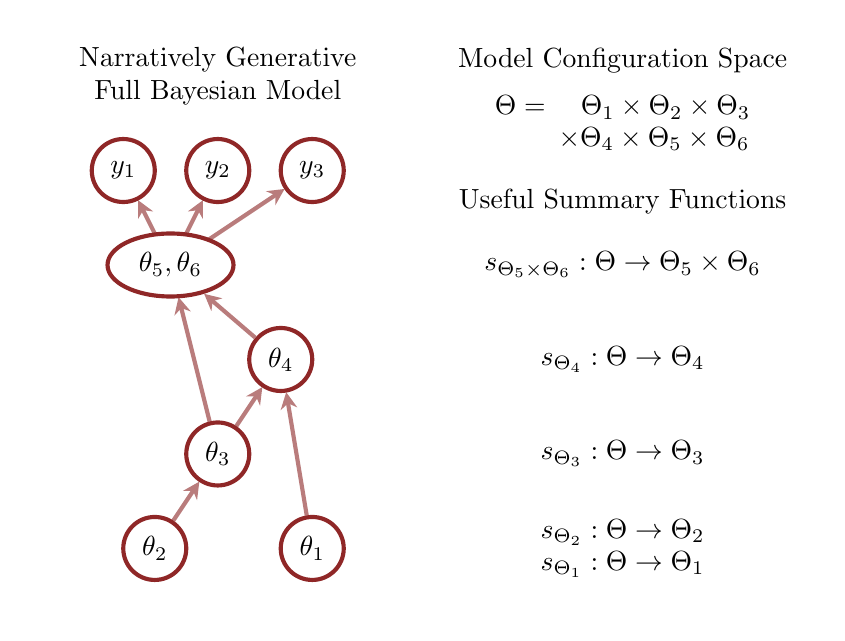
\begin{tikzpicture}[scale=0.2, thick]

  \pgfmathsetmacro{\r}{2}
    
  \begin{scope}[shift={(0, 0)}]
    \draw[white] (-12, 2) rectangle (12, 39);
  
    \node[align=center] at (0, 36) { Narratively Generative\\Full Bayesian Model };
  
    \coordinate (A) at (6, 6);
    \coordinate (B) at (-4, 6);
    \coordinate (C) at (0, 12);
    \coordinate (D) at (4, 18);
    \coordinate (E) at (-3, 24);
    \coordinate (F) at (-6, 30);
    \coordinate (G) at (0, 30);
    \coordinate (H) at (6, 30);

    \foreach \B/\E in {A/D, B/C, C/D, C/E, E/F, E/G, E/H} {
      \draw[-{Stealth[length=6pt, width=6pt]}, shorten <=12.1, shorten >=12, color=mid, line width=1.5] (\B) -- (\E);
    }

    \filldraw[fill=white, draw=dark, line width=1.5] (A) circle (\r)
    node[color=black] { $\theta_{1}$ };

    \filldraw[fill=white, draw=dark, line width=1.5] (B) circle (\r)
    node[color=black] { $\theta_{2}$ };

    \filldraw[fill=white, draw=dark, line width=1.5] (C) circle (\r)
    node[color=black] { $\theta_{3}$ };
    
    \filldraw[fill=white, draw=dark, line width=1.5] (D) circle (\r)
    node[color=black] { $\theta_{4}$ };
    
    \filldraw[fill=white, draw=dark, line width=1.5] (E) circle [x radius={2 * \r}, y radius={\r}]
    node[color=black] { $\theta_{5}, \theta_{6}$ };
    
    \filldraw[fill=white, draw=dark, line width=1.5] (F) circle (\r)
    node[color=black] { $y_{1}$ };
      
    \filldraw[fill=white, draw=dark, line width=1.5] (G) circle (\r)
    node[color=black] { $y_{2}$ };

    \filldraw[fill=white, draw=dark, line width=1.5] (H) circle (\r)
    node[color=black] { $y_{3}$ };

    \foreach \B/\E in {D/E} {
      \draw[-{Stealth[length=6pt, width=6pt]}, shorten <=12.1, shorten >=16, color=mid, line width=1.5] (\B) -- (\E);
    }

  \end{scope}
  
  \begin{scope}[shift={(26, 0)}]
    \draw[white] (-12, 2) rectangle (12, 39);
  
    \node[align=center] at (0, 37) { Model Configuration Space };
    
    \node[align=center] at (0, 34) { $\Theta = \quad \Theta_{1} \times \Theta_{2} \times \Theta_{3}$ };
    
    \node[align=center] at (0, 32) { $\quad\quad\; \times \Theta_{4} \times \Theta_{5} \times \Theta_{6}$ };
         
    \node[align=center] at (0, 28) { Useful Summary Functions };
  
    \node[align=center] at (0, 24) { $s_{\Theta_{5} \times \Theta_{6}} : \Theta \rightarrow \Theta_{5} \times \Theta_{6}$ };
    \node[align=center] at (0, 18) { $s_{\Theta_{4}} : \Theta \rightarrow \Theta_{4}$ };
    \node[align=center] at (0, 12) { $s_{\Theta_{3}} : \Theta \rightarrow \Theta_{3}$ };
    \node[align=center] at (0, 7) { $s_{\Theta_{2}} : \Theta \rightarrow \Theta_{2}$ };
    \node[align=center] at (0, 5) { $s_{\Theta_{1}} : \Theta \rightarrow \Theta_{1}$ };
  \end{scope}

\end{tikzpicture}

\end{document}  